\documentclass{llncs}
\pagestyle{plain}
\usepackage{amsmath,amssymb,amsfonts,stmaryrd}
\usepackage{graphicx}
\usepackage[usenames,dvipsnames]{color}
\usepackage{tikz}
\usepackage{hyperref}
\usepackage[T1]{fontenc}
\usepackage{listings}
\lstset{%
   basicstyle=\ttfamily, %\scriptsize\ttfamily,
%   frame=single,
   breaklines=true,
}
%\usepackage{algorithm}
\usepackage{float}

\newcommand{\wip}[1]{\textcolor{Purple}{WIPWIPWIPWIP #1 WIPWIPWIPWIP}}
\newcommand{\francois}[1]{\textcolor{blue}{#1}}
\newcommand{\sylvain}[1]{\textcolor{green}{#1}}

\newcommand{\defleq}{\sqsubseteq_{\text{def}}}
\newcommand{\lra}{\longrightarrow}

\floatstyle{boxed}
\newfloat{listfig}{htb}{lstfig}
\floatname{listfig}{Listing}

\floatstyle{ruled}
\newfloat{algorithm}{htpb}{algfig}
\floatname{algorithm}{Algorithm}




\begin{document}

\title{Probably Approximately Correct Learning of Regulatory Networks from Time-Series Data}

\author{Arthur Carcano\inst{1} \and Fran\c{c}ois Fages\inst{2} \and Sylvain
Soliman\inst{2}}

\institute{%
Ecole Normale Sup\'erieure, Paris, France\\
  \email{arthur.carcano@ens.fr}
\and Inria, University Paris-Saclay, Lifeware group, France\\
   \email{Francois.Fages@inria.fr},
   \email{Sylvain.Soliman@inria.fr}
}

\maketitle

\begin{abstract}
Automating the process of model building from experimental data 
is a very desirable goal to palliate the lack of modellers for many applications.
Despite the spectacular progress of machine learning techniques in data analytics, classification and clustering,
learning dynamical models from data time-series is challenging.
In this paper we investigate the use of the Probably Approximately Correct (PAC) learning 
framework of Leslie Valiant as a method for the automated discovery of influence models of biochemical processes from Boolean and stochastic traces. 
We show that Thomas's Boolean influence systems can be naturally represented by k-CNF formulae
and learned
from time-series data with a quasi linear number of Boolean activation samples per species,
and that positive Boolean influence systems can be represented by monotone DNF formulae
and learned actively with both activation samples and oracle calls.
We evaluate the performance of this approach on a model of T-lymphocyte differentiation with prior knowledge,
and discuss its merits as well as its limitations with respect to realistic experiments.
\end{abstract}

\section{Introduction}

Modelling biological systems is still an art which is currently limited in its applications by the number of available modellers.
Automating the process of model building is thus a very desirable goal
to attack new applications, develop patient-tailored therapeutics,
and also design experiments that can now be largely automated
with a gain in both the quantification and the reliability of the observations, at both the single cell and population levels.

Machine learning is revolutionising the statistical methods in biological data analytics,
data classification and clustering, and prediction making.
However, learning dynamical models from data time-series is more challenging.
There has been early work on the use of machine learning techniques, such as inductive
 logic programming~\cite{Muggleton95ngc} combined with active learning in the vision of the ``robot scientist''~\cite{BMOKRK01etai},
to infer gene functions,
metabolic pathway descriptions~\cite{AM02etai,AM02slps}
or gene influence systems~\cite{BCRG04jtb},
or to revise a reaction model with respect to CTL properties~\cite{CCFS06tcsb}.
Since a few years, progress in this field can be measured on public benchmarks
of the ``Dream Challenge'' competition~\cite{Meyer14bmc}.
Logic Programming, and especially \emph{Answer Set Programming} (ASP), provide efficient tools such as CLASP~\cite{GKNS07lpnmr}
to implement learning algorithms for Boolean models.
They have been applied in~\cite{GSTUV08iclp} to the detection of  inconsistencies in large biological networks,
and have been subsequentially applied to the inference of gene networks from gene expression data and to the design of discriminant experiments~\cite{VKASSSG15frontiers}.
Furthermore, ASP has been combined with CTL model-checking in~\cite{OPSSG16biosystems} to learn mammalian signalling networks from time series data,
and identify erroneous time-points in the data.

Active learning extends machine learning with the possibility to call oracles, e.g.~make experiments,
and budgeted learning adds costs to the calls to the oracle.
The original motivation for the budgeted learning protocol came from medical applications in which the outcome of a treatment,
drug trial, or control group is known, and the results of running medical tests are each available for a price~\cite{DZBSM13ml}.
In this context, multi-armed bandit methods~\cite{DBSSZ07icdm} currently provide the best strategies.
In~\cite{LMALS14ecml}, a bandit-based active learning algorithm is proposed for experiment design in dynamical system identification.

In this paper, we consider the framework of Probably Approximately Correct (PAC) Learning 
which was introduced by Leslie Valiant in his seminal paper on a theory of the learnable~\cite{Valiant84cacm}.
Valiant questioned what can be learned from a computational viewpoint,
and introduced the concept of probably approximately correct (PAC) learning,
together with a general-purpose polynomial-time learning protocol.
Beyond the learning algorithms that one can derive with this methodology,
Valiant's theory of the learnable has profound implications
on the nature of biological and cognitive processes,
of collective and individual behaviors,
and on the study of their evolution~\cite{Valiant13book}.

Here we investigate PAC learning as a method for the automated discovery of influence models of biochemical processes from time-series data. 
To the best of our knowledge, 
the application of PAC learning to models of biological systems has not been reported before.
We show that Thomas's gene regulatory networks~\cite{Thomas91jtb,Thomas73jtb} can be naturally represented by 
Boolean formulae in conjunctive normal forms with a bounded number of litterals (i.e.~k-CNF formulae),
and can be learned from Boolean transition samples with a quasi linear number of Boolean transition samples, using Valiant's PAC learning algorithm for k-CNF formulae.
We also show that Boolean influence systems with their positive Boolean semantics discussed in~\cite{FMRS16cmsb}
can be naturally represented by monotone DNF formulae.
Valiant's PAC active learning algorithm for monotone DNF formulae makes it possible in theory 
to learn a Boolean influence model from a set of positive examples and a set of calls to an oracle for the Boolean transitions.
However, \dots

These results are illustrated in the following with a Boolean influence model of the lymphocyte T as running example.
They are further evaluated on \dots of size \dots
We evaluate the PAC learning protocols first without prior knowledge, and then with knowledge of the unsigned or signed influence graph without Boolean functions.

\sylvain{will be completed when we know what is in the article or not}

We conclude on the merits of this framework, but also on its limits to scale up,
and to be usable in the context of a wet lab context for real biological experiment design.


\section{Preliminaries on PAC Learning}\label{pac}

\subsection{PAC Learning Protocol}


Let us consider a finite set of Boolean variables $x_1,\ldots,x_n$,
\begin{itemize}
	\item A vector is an assignment of the $n$ variables to $\mathbb{B}_* = \{0,1,*\}$;
	\item A total vector is a Boolean assignment, in $\mathbb{B} = \{0,1\}$;
	\item A Boolean function $G:{\mathbb{B}}^n \rightarrow \mathbb{B}$;
	assigns a Boolean value to each total vector;
\item A concept $F:{\mathbb{B}_*}^n \rightarrow \mathbb{B}$
	assigns a Boolean value to each vector.
\end{itemize}

The idea behind the PAC learning protocol is to discover a concept, or a Boolean function, which approximates a hidden concept $F$, while restricting oneself to the two following operations~:
\begin{itemize}
  \item
\textsc{Sample}$()$: returns a positive example, i.e.~a vector $v$ such that $F(v)=1$.
The output of \textsc{Sample}$()$ is assumed to follow a given probability distribution $D(v)$, which is used to measure the approximation of the result.
  \item
\textsc{Oracle}$(v)$: returns the value of $F(v)$ for any input vector $v$.
\end{itemize}


\begin{definition}[Learnable class~\cite{Valiant84cacm}]\label{def:learnclass}
   A class $\cal M$ of \emph{Boolean functions} is said to be \emph{learnable}
   if there exists an algorithm $\cal A$ such that:
   \begin{itemize}
      \item $\cal A$ runs in polynomial time both in $n$ -- the dimension of the models to learn -- and $h$ the precision parameter;
      \item
         for any function $F$ in $\cal M$, and any distribution $D$ on the positive examples,
         $\cal A$ deduces with probability higher than $1-h^{-1}$ an approximation $G$ of $F$ such that
         \begin{itemize}
            \item $G(v)=1$ implies $F(v)=1$ (no false positive)
            \item
               $\displaystyle\sum_{v\ s.t.\ F(v)=1\wedge G(v)=0} D(v) < h^{-1}$ (low probability of false negatives)
         \end{itemize}
   \end{itemize}
\end{definition}

For the sake of simplicity, the same precision parameter $h$ is used above for quantifying both the probability that the result is correct,
and the error tolerated in the correctness criterion.

We could have also removed the distinction between concepts and Boolean functions here,
since in the sequel we will learn Boolean functions only, and obtain samples from data time series which provide total vectors.
We keep the distinction in this section for the sake of generality.

\subsection{PAC Learning Algorithms}

Valiant showed the learnability of some important classes of functions in this framework,
in particular for Boolean formulae in conjunctive normal forms with at most $k$ literals per conjunct (k-CNF),
and for monotone (i.e.~negation free) Boolean formulae in disjunctive normal form (DNF).

The computational complexity of the PAC learning algorithms for these classes of functions is expressed in terms of the function
$L(h,S)$ defined as the smallest integer $i$ such that
in $i$ independent Bernoulli trials, each with probability at least $h^{-1}$ of success, the probability of having fewer than $S$ successes is less than $h^{-1}$.
Interestingly, this function is quasi-linear in $h$ and $S$, i.e.~for all
integers $S\ge 1$ and reals $h>1$, we have $L(h,S) \le 2h(S+\log_e h)$~\cite{Valiant84cacm}.

\begin{theorem}[\cite{Valiant84cacm}]\label{thm:kcnf}
For any $k$, the class of $k$-CNF formulae on $n$ variables is learnable with an
algorithm that uses $L(h,{(2 n)}^{k+1})$ positive examples and no calls to the
oracle.
\end{theorem}

The proof is constructive and relies on Alg.~\ref{algCNF} below. In this algorithm, the initialization of the learned function $g$ to the false constraint expressed as the conjunction of all possible \emph{clauses} (i.e.~disjunctions of litterals)
leads to the learning of a minimal generalization of the positive examples with mainly no false positive and low probability of false negatives.

\begin{algorithm}
\begin{enumerate}
  \item initialise $g$ to the conjunction of all possible clauses of at most $k$ literals (there are ${(2n)}^k$ such clauses),
\item do $L(h,(2n)^{k+1})$ times 
\begin{enumerate}
\item $v:=\textsc{Sample}()$
\item delete all the clauses in $g$ that do not contain a literal true in $v$
\end{enumerate}
\item output: $g$
\end{enumerate}
\caption{PAC-learning of $k$-CNF formulae.\label{algCNF}}
\end{algorithm}

In our implementation of the PAC-learning algorithm for $k$-CNF formulae,
we make use of the lattice structure of $k$-clauses ordered by implication.
It is worth remarking that this data structure allows
\begin{itemize}
	\item $O(1)$ access to any $k$-clause
	\item and for a clause $c$, $O(1)$ access to the smallest clauses implied by $c$ and to the biggest clauses that imply $c$.
\end{itemize}

Monotone DNF formulae are also learnable.
Let the \emph{degree} of a Boolean formula be the largest number of prime
implicants in an equivalent rewriting of the formula as a non-redundant sum of
prime-implicants~\cite{Valiant84cacm}.


\begin{theorem}[\cite{Valiant84cacm}]\label{thm:mdnf}
    The class of monotone DNF formulae on $n$ variables is also learnable with an
    algorithm that uses $L(h,d)$ examples and $d n$ calls to the oracle,
    where $d$ is the \emph{degree} of the function to learn.
\end{theorem}

The proof relies on Alg.~\ref{algDNF}. As previously, the algorithm guarantees that a minimal generalization is learned from both the samples and the oracle.

\begin{algorithm}
\begin{enumerate}
\item initialise $g$ with false (constant zero),
\item
do $L(h,d)$ times 
\begin{enumerate}
\item $v:=\textsc{Sample}()$
	\item 
	if $v\Rightarrow g$ exit
\item for $i:=\ 1\ to \ n$
\begin{enumerate}
\item if $x_i$ is determined in $v$
\begin{enumerate}
\item $v^*:=v[x_i\leftarrow *]$
\item if $\textsc{Oracle}(v^*)$ then 
\begin{itemize}
\item $v:=v^*$
\item $m:=\bigwedge_{v\Rightarrow x_j} x_j\wedge\bigwedge_{v\Rightarrow\neg x_k}\neg x_k$ 
\item $g:=g\vee m$
\end{itemize}
\end{enumerate}
\end{enumerate}
\end{enumerate}
\item output: $g$
\end{enumerate}
\caption{PAC-learning of monotone DNF formulae.\label{algDNF}}
\end{algorithm}

The polynomial computational complexity follows from the fact that each monomial $m$ is a prime implicant
of $f$ by construction, and that it is constructed by at most $n$ calls to the
oracle.




\section{Influence Models of Molecular Cell Processes}

\francois{I tried to import our definitions but the stochastic-Boolean semantics used in this paper is a bit different\dots}

\francois{The good point with starting with influence systems instead of directly Thomas networks
is that we can show ``realistic'' stochastic simulations and understand later Thomas's logical functions
which otherwise would be quite strange to present on this simple example}


In this section, we present four Boolean formalisms used to model regulatory networks in cell molecular biology.
%and to which we will later whether or not PAC learning is applicable.
We assume a finite set of molecular species $\{x_1,\dots,x_n\}$ 
and consider Boolean states that represent the activation or presence of each molecular species of the system, 
i.e.~total vectors in $\mathbb{B}^n$ that specify whether or not the $i$th species is present, or the $i$th gene activated.

\subsection{Influence Systems with Forces}


Influence systems with forces have been introduced in~\cite{FMRS16cmsb}
to generalize the widely used logical models of regulatory networks \emph{\`a la} Thomas~\cite{Thomas73jtb} 
in order to provide them with a hierarchy of semantics
including differential, stochastic, Petri Net and Boolean semantics.

\begin{definition}\cite{FMRS16cmsb}
An \emph{influence system}
   $I$ is a set of quintuples $(P, I, t, \sigma, f)$ called \emph{influences},
   where 
\begin{itemize}
\item $P$ is a multiset on $S$, called \emph{positive sources} of the influence, 
\item $I$ a multiset of \emph{negative sources}, 
\item $t\in S$ is the \emph{target},
\item $\sigma\in\{+,-\}$ is the \emph{sign} of the influence, accordingly called either \emph{positive or negative influence},
\item and $f:\mathbb{R_+}^n\to\mathbb{R}$, called the \emph{force} of the influence,
is a partially differentiable function, non-negative
   on $\mathbb{R}_+^n$;
\item $x_i\in P$ if and only if $\sigma = +$ (resp.\ $-$) and
   ${\partial {f}}/ {\partial x_i}(\vec x)>0$ (resp.\ $<0$) for some value
   $\vec x\in\mathbb{R}_+^n$;
\item $x_i\in I$ if and only if $\sigma = +$ (resp.\ $-$) and
   ${\partial {f}}/ {\partial x_i}(\vec x)<0$ (resp.\ $>0$) for some value
  $\vec x\in\mathbb{R}_+^n$;
\end{itemize}
\end{definition}

We distinguish the positive sources from the negative sources of an influence (positive or negative),
in order to annotate the fact that in the differential semantics,
the source increases or decreases the force of the influence,
and in the Boolean semantics with negation whether the source or the negation of the source
is a condition for a change in the target.

In the examples below, we use the ASCII syntax of Biocham v4 for influences.
Positive (resp.~negative) influences are written with an arrow \lstinline|->| (resp.~\lstinline+-<+)
which separates the sources from the target.
The positive and negative sources are separated
by a \lstinline|/|, which can be omitted if there is no negative source.

\begin{example}\label{ex:LVi}
   The classical birth-death model of Lotka--Volterra can be represented by the following
influence system between a proliferating prey $A$ and a predator $B$,
where the influence forces are used for stochastic simulation:
  \lstinputlisting[firstline=6,lastline=9]{examples/LVif.bc}

\vspace{-2cm}\hfill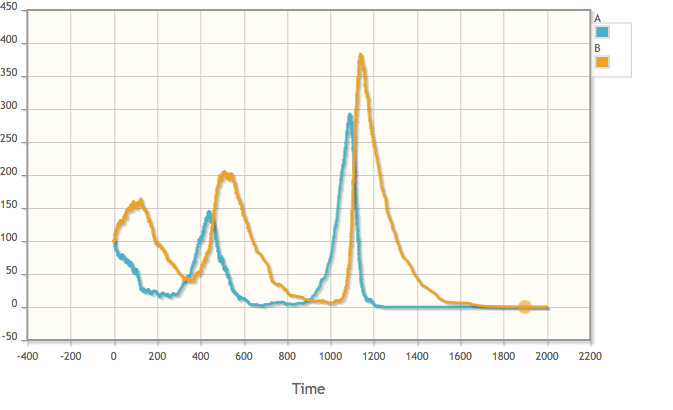
\includegraphics[width=0.45\textwidth]{LVstoch.png}
   composed of four influences with no negative sources:
   $(\{A, B\}, \emptyset, A, -, k1*A*B)$, $(\{A, B\}, \emptyset, B, +, k1*A*B)$, $(\{A\}, \emptyset, A, +, k2*A)$ and $(\{B\}, \emptyset, B, -, k3*B)$.
This example contains both positive and negative influences but no influence inhibitor, i.e.~no negative source in the influences.

For an example of influence with inhibitor, one can consider the specific inhibition of the proliferation rate of $A$ by some variable $C$
which is distinguished from a general negative influence of $C$ on $A$, by writing $C$ as an inhibitor of the positive influence of $A$ on $A$:
   \begin{lstlisting}
k2*A/(1+C) for A/C -> A.
   \end{lstlisting}
\end{example}

While it may seem natural in the Boolean semantics of an influence system to interpret the negative sources by negations
for the enabling conditions for applying an influence in a given state, 
the approximation and abstraction relationships that link the different semantics of a given influence system,
lead us to consider the positive semantics of influence systems which simply ignores the negative sources~\cite{FMRS16cmsb}.
Here, we adopt the Boolean semantics with negation and consider the particular case of \emph{positive influence systems}
which may contain positive and negative influences but only positive sources no negative sources.


\begin{definition}[Boolean Semantics]
   The Boolean semantics of an influence system $\{(P_i, I_i, t_i, \sigma_i,
   f_i)\}_{1\leq i\leq n}$
   over a set $S$ of $n$ variables,
   is the Boolean transition system $\lra$ defined over Boolean state total vectors in $\mathbb{B}^n$
   by
   ${\vec x}\lra{\vec x'}$ if there exists an influence $(P_i, I_i, t_i, \sigma_i, f_i)$
   such that ${\vec x}\models \bigwedge_{p\in P_i}$
   and ${\vec x'} = {\vec x}\ \sigma_i\ t_i$.
\end{definition}

The stochastic semantics with negation is as follows:

\begin{definition}[Stochastic Semantics]\label{def:stoch}
   The stochastic semantics of an influence system $\{(P_i, I_i, t_i,
   \sigma_i, f_i)\}_{1\leq i\leq n}$ over a set $S$ of $n$ variables, relies
   on the transition system $\lra$ defined over discrete states, i.e.\
   vectors in $\mathbb{N}^n$, by $\forall (P_i, I_i, t_i, \sigma_i, f_i), {\vec
   x}\lra{\vec x'} \text{ with propensity }f_i\text{ if }{\vec x}\geq P_i,
   {\vec x}<I_i$ and ${\vec x'} = {\vec x}\  \sigma_i\ t_i$

   Transition probabilities between discrete states are obtained through
   normalization of the propensities of all enabled transitions, and the time
   of next reaction can also be given \emph{\`a la}
   Gillespie~\cite{Gillespie77jpc}.

\end{definition}

\subsection{Monotone DNF Representation of Positive Influence Systems}


In this section we restrict ourselves to the positive semantics of influence systems
and syntactically to influence systems without inhibitors, as in the beginning
of Ex.~\ref{ex:LVi}.
\sylvain{Not sure we need this syntactic restriction here}
Because of this restriction, we shall write the influences as 4-tuples instead
of 5-tuples by ignoring $I$.

\begin{definition}[Positive Boolean Semantics]
	The positive Boolean semantics of an influence system $\{(P_i, t_i,
   \sigma_i, f_i)\}_{1\leq i\leq n}$
	over a set $S$ of $n$ variables,
	is the Boolean transition system $\lra$ defined over Boolean state total vectors in $\mathbb{B}^n$
	by
	${\vec x}\lra{\vec x'}$ if there exists an influence $(P_i, t_i, \sigma_i, f_i)$
	such that ${\vec x}\models \bigwedge_{p\in P_i}$
	and ${\vec x'} = {\vec x}\ \sigma_i\ t_i$.
\end{definition}

Positive influence systems may hence be represented as $n$ activation and $n$ deactivation functions, which are defined as follows:


\begin{definition}\label{def:activation}
	Given a network of $n$ genes $x_1,\ldots,x_n$, and
	an integer $1 \leq k \leq n$ we can define ${x_k}^+$ (resp.\ ${x_k}^-$):
	${\{0,1\}}^n \rightarrow\{0,1\}$ the activation (resp.\ deactivation)
	Boolean function of $x_k$. In a given state $v$, ${x_k}^+(v)$ (resp.\
   ${x_k}^-(v)$) is worth 1 if and only if the gene $x_k$ can be activated
   (resp.\ deactivated) from state $v$.
\end{definition}

The representation of (de)activation functions by an influence system 
corresponds to a decomposition of the formulae in DNF, 
with one influence per disjunct and one source per conjunct.
Furthermore, the restriction to \textbf{positive} influence systems, leads to monotone DNF formulae.

\begin{example}

For Ex.~\ref{ex:LVi} we would have as monotone DNF formulae:
\begin{eqnarray*}
   A^+&=&(A)\\
   A^-&=&(A \wedge B)\\
   B^+&=&(A\wedge B)\\
   B^-&=&(B)
\end{eqnarray*}

\end{example}

%Note that in Ex.~\ref{ex:lympho} no (de)activation function is monotone.

\subsection{$k$-CNF Representation of Influence Systems}

Monotone DNF formulae cannot encode the Boolean dynamics of influence systems with inhibitors, which test by negation the absence of negative sources.
This is possible using the $k$-CNF representation of the system, which constrains not the absence of inhibitors but the number of species that can play a given ``role''. To be more precise, let's consider the following CNF for a hypothetic influence:

\[
\left(a \vee b \vee c\right) \bigwedge
\left(d \vee e\right) \bigwedge 
\neg f
\]

Then each of the clause can be interpreted as a role, and for the activation of our hypothetic gene, we need at least one species that plays this role. For example, the enzyme can be $a$, $b$, or $c$ whereas 
the reactant is $d$ or $e$, and we need that $f$ be inactive.


\begin{example}
   The Lotka--Volterra example Ex.~\ref{ex:LVi} with inhibition cannot be
   translated to a monotone DNF formula. It has however the following CNF
   representation. It is easy to
   notice that $k=1$ is enough since there is only one positive and one
   negative influence for each target.
\begin{eqnarray*}
   A^+&=&(A)\wedge(\neg C)\\
A^-&=&(A) \wedge (B)\\
B^+&=&(A)\wedge (B)\\
   B^-&=&(B)
\end{eqnarray*}

\end{example}

\begin{example}
   In Ex.~\ref{ex:lympho} we can see for instance that there is a 2-CNF
   representation:
   \[\text{IFNg}^+=(\text{STAT4}\vee \text{TBet})\qquad
   \text{IFNg}^-=(\neg \text{STAT4})\wedge(\neg \text{TBet})\]
\end{example}

\subsection{$k$-CNF Models of Thomas's Regulatory Networks}

The $k$-CNF representation also fits the Boolean semantics of Thomas's gene
regulatory networks~\cite{Thomas73jtb}.

\begin{definition}
   A \emph{Thomas} network is defined by a set of genes $\{x_1,\dots,x_n\}$
   and $n$ Boolean functions $\{f_1,\dots,f_n\}$ describing for each gene its
   possible next state, given the current state.
\end{definition}

$k$-CNF formulae can be used to represent such gene regulatory network functions with some reasonable restrictions on their connectivity.
In particular, it is worth noticing that in Thomas networks of degree bounded by $k$,
each gene has at most $k$ regulators, each gene activation function $f_i$ thus depends of at most $k$ variables
and can certainly be represented by a $k$-CNF formula.

As proven in~\cite{FMRS16cmsb}, in the Boolean setting any influence system is
also a Thomas' network.
As this will be useful later on, we also remark that the Thomas' Network can
be computed from the (de)activation functions presented in Def.~\ref{def:activation} by:

\[
\forall 1 \leq i \leq n, \forall v, f_i(v) = \left\{\begin{array}{l}
1 \text{ if } \left\{\begin{array}{l}
v_i = 0 \text{ and } {x_i}^+(v) = 1\\
v_i = 1 \text{ and } {x_i}^-(v) = 0 \\
\end{array}\right.\\[1em]
0 \text{ if } \left\{\begin{array}{l}
v_i = 0 \text{ and } {x_i}^+(v) = 0\\
v_i = 1 \text{ and } {x_i}^-(v) = 1\\
\end{array}\right.
\end{array}\right.
\]

\begin{example}
   We can apply the above translation to our Lotka--Volterra example of
   Ex.~\ref{ex:LVi}. We obtain:
   \begin{eqnarray*}
   f_A &=& A \wedge\neg B\\
   f_B &=& 0
   \end{eqnarray*}

   Note that the form of $f_B$ only means that the only possible state change
   for $B$ is from $1$ to $0$. Of course $B$ can also stay at $1$ but
   non-terminal self-loops do not appear in such a logical model.
\end{example}

\begin{example}
   Ex.~\ref{ex:lympho} is originally a Thomas' network, where we have, for
   instance:
   \[f_\text{IFNg}=(\text{STAT4}\vee \text{TBet})\]
\end{example}

\section{PAC Learning from Traces} %Experimental Setup}

%To further discuss the applicability of PAC learning to actual experiments, we hereby introduce what we believe is a plausible experimental setup, and discuss its implications on the learning of different classes of functions.

\subsection{Steps and Traces}

From now on, we do not assume %anymore 
that we have full access to the hidden Boolean function for
\textsc{Sample} and \textsc{Oracle}, but we restrict ourselves to the observations that can be obtained from data time-series, or traces,
produced either from real biological experiments, or, for the purpose of evaluating the learning method, from simulations.

\begin{figure}[htbp]
	{\large 
	\[
	\cdots
	\rightarrow
	\underset{\vspace{1em}(a)}{
		\left(\begin{array}{c}
		0\\ 1\\ 0\\ 1
		\end{array}\right)}
	\rightarrow
	\underset{\vspace{1em}(b)}{
		\left(\begin{array}{c}
		\textbf{\textit{1}}\\ 1\\ 0\\ 1
		\end{array}\right)}
	\rightarrow
	\underset{\vspace{1em}(c)}{
		\left(\begin{array}{c}
		1\\ 1\\ 0\\ \textbf{\textit 0}
		\end{array}\right)}
	\rightarrow
	\cdots
	\]
}
	\caption{\label{steps}Illustration of our hypothetical experimental setup with three steps of a trace. Between $a$ and $b$, the first gene has been activated, and between $b$ and $c$, the last one has been deactivated.}
\end{figure}

More specifically, and as illustrated in figure~\ref{steps}, we consider that our experimental setup enables us to identify a ``step'' of its evolution, i.e.~that we are able to obtain a trace $(v_i)_{0 \leq t \leq T}$ of the Boolean state of activation of its species where for all $t$ in $[0,T-1]$, $v_t$ and $v_{t+1}$ differ in exactly one coordinate. That is, the state of exactly one species has changed.


Even though we will finally not require it, we first also consider that our experimental setup enables us to put the system in a given state, i.e.~that for any $v \in \mathbb{B}^n$ we can set the experiment's initial conditions so that they are correctly abstracted by $v$.

\subsection{Application of PAC Learning on Transition Traces}
%Now that our hypothetical experimental setup is described, we will discuss how the two key operations of PAC-learning (\textsc{Sample} and \textsc{Oracle}) can be implemented, if at all, in it.

Because both influence systems and \textit{\`{a} la Thomas} networks essentially boil down to activation and deactivation functions we limit ourself to those in the following.

\subsubsection{Sampling}

We can first remark that sampling of (de)activation function is straightforward in this setting. Referring to figure~\ref{steps}, $(a)$ is a positive example for the activation function ${x_1}^+$, and $(c)$ for ${x_4}^-$.

A call to \textsc{Sample} can then simply be a search in the trace for the next positive example for the current function. Issues \wip{that have not been studied yet} may arise if there is not enough samples to guarantee a good approximation. 
%Our belief is 
We assume here that those issues can be solved by running several traces from different initial states.

\subsubsection{Oracle}
The \textsc{Oracle} function needs to evaluate the (de)activation function on a given total vector $v$, that is, it needs to be able to set the system in a state abstracted by $v$ and say whether or not a given gene can be (de)activated from this state.

The intuitive solution is the following : set the system in the desired state and see whether or not the gene is (de)activated. 
However, different atomic steps are possible from a given state and we have no guarantee that the one we are interested in will happen
in several runs of the experiment. 

Moreover, in its simple form presented above, %the current state of 
Valiant's framework does not allow for the oracle to be probabilistic.
In practice however, since we cannot run this ``state and observe the first atomic step'' scheme an infinite number of time to be able to tell that the (de)activation can only happen with probability 0,
we have to content ourself with an imperfect oracle.
%A peculiarly fast-thinking reader may also have notice that different (and often infinitely many) states of the system may also be abstracted by the same Boolean total vector $v$, and that the transition may also happen from only some of them.
%For those reasons, algorithm requiring the \textsc{Oracle} function seem not applicable as of today, and we choose to only focus on $k$-CNF and sampling from now on.


%\section{In sillico application}
\subsection{PAC Learning from Boolean Traces}

\francois{To update since the example has already been introduced before}

A first experimentation was to simulate Boolean traces for a given influence network, and use them as a basis to learn. 
A toy example is given in listing~\ref{bool-LV} (influence network) and the corresponding results are presented in listing~\ref{bool-LV.res}.

In output \texttt{!A} means $\neg A$ or ``not A''.

\subsubsection{Results}

\begin{listfig}[htp]
	\lstinputlisting{examples/bool-lokta.reac}
	\caption{An influence system describing the Lokta-Voltera prey vs.\ predator model. Numbers in parenthesis indicate the force of an influence.\label{bool-LV}}
\end{listfig}
\begin{listfig}[htp]
	\lstinputlisting{examples/bool-lokta.res}
	\caption{Results of PAC-learning on traces of the Boolean simulation of the Lokta-Voltera toy example.\label{bool-LV.res}}
\end{listfig}

The results can be interpreted as follow:

Both the predator and the prey species cannot appear. It is important to note that the activation functions in the Lokta Voltera models means the apparition on extinction of the species as a whole and not of individuals of it.

For the predator to disappear, it is necessary that there is predator in the first place and that there is no prey. If the first part of this conjunction is obviously true, the second is false: strictly speaking, predators may disappear even if there is prey left, yet this case is very unlikely: the most likely case is that the predator will go extinct only once there are no more preys left for it to eat. This is a good example of how the learning is only approximate.

Finally, for the prey to go extinct, there must be both prey in the first place and predator to eat it. This is true.

\subsubsection{On the quantification of the approximation}

As it can be seen even on this very simple example, the "approximately" in "probably approximately correct" is not there for nothing. Yet, as explained in definition~\ref{def:learnclass}, the quantification of this approximation relies on the knowledge of the distributions of the samples.

Even though we were not able to write it down exactly, it is our conjecture that in the present case, the probability of a positive example $v$ of (de)activation function $x\pm$ to be sampled is strongly and intuitively correlated to both the probability that the system reaches state $v$ and the probability of the actual (de)activation of gene $x$ from state $v$. 



\subsection{PAC Learning from Stochastic Traces}

Let us now consider traces not directly produced from a Boolean model, but from more realistic data time series.
For the sake of evaluating the learning method,
we generate stochastic traces from the hidden model, using Gillespie's
algorithm for the simulation of the stochastic semantics given in
Def.~\ref{def:stoch}.

The traces obtained are in ${\mathbb{N}}^n$, they are then abstracted to
Boolean traces over ${\mathbb{B}}^n$ by the usual $\{0, >0\}$ abstraction.

It would also be possible to try and learn directly a Boolean model from
stochastic traces (using $x_i\lra x_i+1$ (resp.\ $x_i-1$) as positive example for the
activiation (resp.\ deactivation)), but since the abstraction of the state
remains necessary we present here a fully abstracted method.

\sylvain{Arthur, can you confirm what is written above?}

\begin{listfig}[hp]
	\lstinputlisting{examples/test.reac}
	\caption{A test reaction, A and E appear naturally in the medium, and A can be turned into B in absence of E. B  can be turned into C. All of the species can disappear due to dilution.\label{test}}
\end{listfig}
\begin{listfig}[hp]
	\lstinputlisting{examples/test.result}
	\caption{Results for the test example\label{test_res}}
\end{listfig}


We ran two example reactions, given in listings~\ref{test}, and~\ref{preypred}. As indicated in listing~\ref{test_res}, the first example gave perfect results.

\begin{listfig}[hp]
	\lstinputlisting{examples/lokta.reac}
	\caption{A Prey-Predator model. The first line indicates the starting quantities for each species. This corresponds to the influence model given in figure~\ref{bool-LV}.\label{preypred}}
\end{listfig}
\begin{listfig}[hp]
	\lstinputlisting{examples/lokta.result}
	\caption{Results for the Prey-Predator model\label{preypred_res}}
\end{listfig}
\francois{Non je ne suis pas d'accord avec ce discours sur les erreurs typiques,
mieux vaudrait parler de sensibilite aux conditions initiales des simulations
en jouant avec quelques experiences sur les nombres initiaux respectifs de proies et predateurs
car les ``erreurs'' d'apprentissage seront differentes,
et si on intègre ces simulations avec differentes conditions initiales on peut espérer me semble-t-il apprendre le bon modele}

\francois{Arthur peux-tu refaire ces experiences?}

As previously, the prey-predator example (listing~\ref{preypred_res}) highlights how dependent to the traces the learned model is.
To further detail this, it is necessary to dive into the Markov chain of the prey-predator stochastic process. A simplification of it is given in figure~\ref{fig:mc-lv}. One can remark that state (2) is an equilibrium state, whereas state (0) is terminal. Because most of the experiments will start in state (3), we can highlight two possible paths, A and B, leading respectively to (2) and (0). Because (de)activation (and hence sample) only comes from a changing of node in fig.~2, each of these pathways result in a different resulting model.

\begin{figure}[htpb]
	\centering
	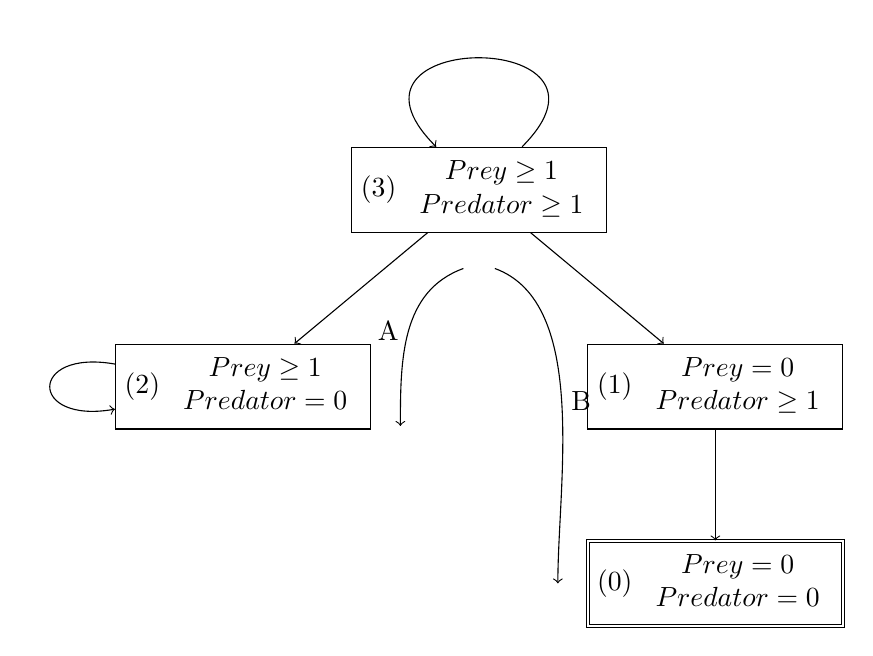
\begin{tikzpicture}
	\path (5,10) node[draw](3) {(3) $\begin{array}{c}
		Prey \geq 1 \\ Predator \geq 1
		\end{array}$}
	(8,7.5) node[draw](1) {(1) $\begin{array}{c}
		Prey = 0 \\ Predator \geq 1
		\end{array}$}
	(2,7.5) node[draw](2) {(2) $\begin{array}{c}
		Prey \geq1 \\ Predator = 0
		\end{array}$}
	(8,5) node[draw,double](0) {(0) $\begin{array}{c}
		Prey = 0 \\ Predator = 0
		\end{array}$}
	;
	\draw [->] (3) -> (2);
	\draw [->] (3) -> (1);
	\draw [->] (1) -> (0);
	\path (3) edge[->,looseness=5] (3);
	\path (2) edge[->,looseness=5,out=170,in=190] (2);
	\draw (4.8,9) edge[->,looseness=1,out=200,in=90] node[below,left] {A} (4,7);
	\draw (5.2,9) edge[->,looseness=0.8,out=-20,in=90] node[below,right] {B} (6,5);
	\end{tikzpicture}
	\caption{A simplification of the markov chain of the Lokta-Voltera process. Probabilities are not given but all arrows have non-null probability to be taken.\label{fig:mc-lv}}
\end{figure}

For A this is:
\begin{verbatim}
Predator+ : False
Predator- : Predator /\ Prey
Prey+ : False
Prey- : False
\end{verbatim}

For B this is:
\begin{verbatim}
Predator+ : False
Predator- : Predator /\ !Prey
Prey+ : False
Prey- : Predator /\ Prey
\end{verbatim}

Both those learned model are not complete, as the sampling will by design miss some of the possible positive examples because only one of A and B paths can be followed.

Indeed, the only way to get the correct result is to run several time the experiment, and hope that probabilities favor us enough so that we have samples from pathways A and B.

Result of such run will then be correct, as illustrated below:
\begin{verbatim}
Predator+ : False
Predator- : Predator
Prey+ : False
Prey- : Predator /\ Prey
\end{verbatim}

\section{Evaluation on a Model of T-helper Lymphocytes Differentiation}\label{ex:lympho}

%All the systems proposed so far were of humble size. 

\subsection{Boolean Thomas Network}

In this section we evaluate the performance of the $k$-CNF PAC learning
algorithm on an influence system of 12 variables and 32 influences that models
the differentiation of the T-helper lymphocytes.

This model, presented in~\cite{RRMTC06tcsb} is actually a Boolean
simplification of the original multi-level model
of~\cite{Mendoza06biosystems}. It studies the regulatory network of stimuli
leading to differentiation between Th-1 and Th-2 lymphocytes from an original
CD4+ T helper (Th-0).

The model has three different stable states corresponding to Th-0 (naive
lymphocyte), Th-1 and Th-2 when IL12 is off, and two others when IL12 is on
(the Th-0 one is lost).

\begin{figure}[htbp]
   \centering
   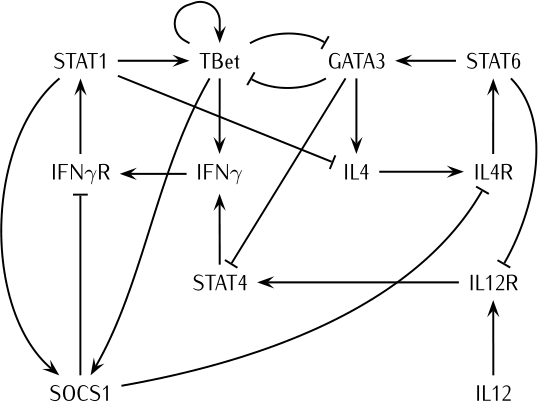
\includegraphics[width=0.8\textwidth]{th_net_clean.png}
   \caption{Fig.~4 of~\cite{RRMTC06tcsb} displaying the Th-lymphocyte
   differentiation model.\label{fig:lympho}}
\end{figure}

Fig.~\ref{fig:lympho} shows the influence graph of the model. The
corresponding code is given in appendix (Listing~\ref{bool-lympho}).

\subsection{Ab initio PAC Learning from Boolean Traces}

\francois{Ce paragraphe ne veut pas dire grand chose --
quel est le probleme exactement?
-- j'ai l'impression que le probleme est juste de ne pas avoir fait assez de runs avec des etats initiaux differents
-- il faudrait le faire pour analyser les resultats et etre plus precis}

However, results of learning on the traces resulting from the Boolean simulation of this system gave very poor results. By this, we mean not that they were bad at predicting the behavior of the model (because guarantees on this come directly from Valiant's work) but that they were hardly readable and of little help to the human experimenter. 
%Thankfully, the PAC learning algorithm for $k$-CNF can be modified to be able to take hints into account.

\subsection{PAC Learning with Prior Knowledge on the Influence Graph}

\francois{donner les temps d execution en precisant sur quelle machine, le nombre de traces, l horizon temporel }

\francois{car les resultats en dependent! il faut donc preciser ces conditions experimentales}

\francois{il faut penser a decrire une recherche reproductible}


Machine learning with prior knowledge can save a lot of work by constraining the possible results and pruning the search.

What we mean by hints can be formally defined: we want the user to be able to specify, for each gene $x$, a set of gene $V_x$ which are the only ones on which $x^+$ and $x^-$ may depend. If one views the influences as a graph, this is akin to specifying a set of possible (undirected) edges outside of which the algorithm cannot build its influence system. Example of such hints for the lymphocyte model are given in listing~\ref{hints}. It is remarkable than when given such hints, the model becomes fully readable for the experimenter, and provides them with information on the exact structure of the influences (as indicated in listing\ref{hints.res}).

\begin{listfig}[htb]
	\lstinputlisting{examples/lympho.hints}
	\caption{Hints for the lymphocyte model. For each species, a set of possible influencers is given. The PAC algorithm will then learn a model in which only the specified influencers can either induce or inhibit the species.\label{hints}}
\end{listfig}



\begin{listfig}
	\lstinputlisting{examples/lympho-bool.res}
	\caption{Results for lymphocyte model, with hints.\label{hints.res}}
\end{listfig}


\section{Active Learning of Positive Influence Systems}
\label{sec:oracles}

\sylvain{I guess this is where the oracle as experiment-design discussion will
take place\dots}

\francois{On va mettre ces considerations en conclusion/perspectives probablement}

The (positive) Boolean semantics of biochemical influence systems
can be directly represented by the disjunction of the (positive) enabling conditions of each, either positive or negative, influence on a given target,
i.e.~by a monotone DNF formula for each activation or inhibition of each target.
In the Lotka--Volterra influence system, the algorithm above is thus expected to learn the structure of the influence system
(without the stochiometry of course),
from the observation that the prey can disappear only in presence of the predator
while the predator can always disappear in presence or absence of the prey.

  Learning reaction models from observed transitions is much more tricky,
  since some reactions may change the Boolean value of several reactants or products in one single transition.
%  Let us first remark that the transition relation $r(x_1,\ldots,x_n,x'_1,\ldots,x'_n)$
%  is naturally represented in DNF by the disjunction of the conjunctions associated to each reaction
%  (remember that there can be several Boolean transitions associated to one reaction for taking
%into account the possibly partial or total consumption of the reactants).
%  is monotonic in the predecessor variables $x_i$'s in the postive Boolean semantics of reactions.
%  Furthermore it is also monotonic in the successor variables $x'_j$ since we consider
%  all partial or total consumptions of reactants.
  Therefore, it is not only the activation and inhibition functions of each species which are to be learnt,
  but the update functions of pairs and triples of species if we restrict to elementary reactions with at most two reactants or products.
  In this case, the update functions can be represented by monotonic DNF formulae, since the (positive) Boolean semantics of a reaction system does not test the absence.
Furthermore,   one cannot expect to learn the structure of such a reaction network
from the observation of the state transitions from one single initial state.
The learning algorithms assumes that the positive examples of the state transition relation be distributed
among the whole vector space.
For instance, in the MAPK example, in addition to the initial state of the wild type organism where all the kinases and phosphatases are present,
it is necessary to consider some mutated organisms, in which some kinases or phosphatases are absent,
in order to gain information on the precise conditions of activation and deactivation of the different forms of the kinases.
This strategy is essentially similar to what the biologists do to elucidate the structure of biological processes
in a qualitative manner.


\section{Conclusion}

In conclusion, we have shown that Valiant's work on PAC learning provides an elegant trail to serve as a way to automatically discover possible regulatory networks of a biological process, given sufficiently precise traces of its run.
When dimension increases, PAC learning algorithms can also leverage available prior knowledge on the system to deliver results.
Moreover, the use of oracles for monotone DNF formulae is of interest to create an online learning algorithm
and is relevant to experimental design.

More work is needed however to make comparisons on common benchmarks
with  other approaches already investigated in this context, such as Answer Set Programming (ASP) and budgeted learning,
and to investigate the applicability to real experiments with particular biological technology.

\bibliographystyle{splncs03}
\bibliography{contraintes}
\newpage
\section*{Appendix}
\begin{listfig}[H]
\lstinputlisting{examples/lympho-bool.reac}
\caption{Code for the lymphocyte differentiation of example~\ref{ex:lympho}.\label{bool-lympho}}
\end{listfig}

\end{document}
